\documentclass[review,onefignum,onetabnum]{siamart190516}

\usepackage[margin=1in]{geometry}
\usepackage{graphicx}
\usepackage{amsfonts}

% Add a serial/Oxford comma by default.
\newcommand{\creflastconjunction}{, and~}

% Sets running headers as well as PDF title and authors
\headers{On Random Noise}{L. Olson}

\title{On Random Noise\thanks{Submitted to the editors April 29, 2021.
\funding{This work was funded by CSE.}}}

\author{Luke N. Olson\thanks{Computational Science and Engineering, University of Illinois at Urbana-Champaign,
(\email{lukeo@illinois.edu}, \url{https://cse.illinois.edu}).}}

\begin{document}

\maketitle

\begin{abstract} This paper is about random noise.
\end{abstract}

\begin{keywords}
  random, noise
\end{keywords}

% REQUIRED
\begin{AMS}
  65N
\end{AMS}

\section{Introduction}

Random noise is an important concept and is best described as a combination of random frequencies.  Take for example~\cref{fig:exp_with_noise}.  Here we see random noise on an exponential.
%
\begin{figure}[!ht]
  \centering
  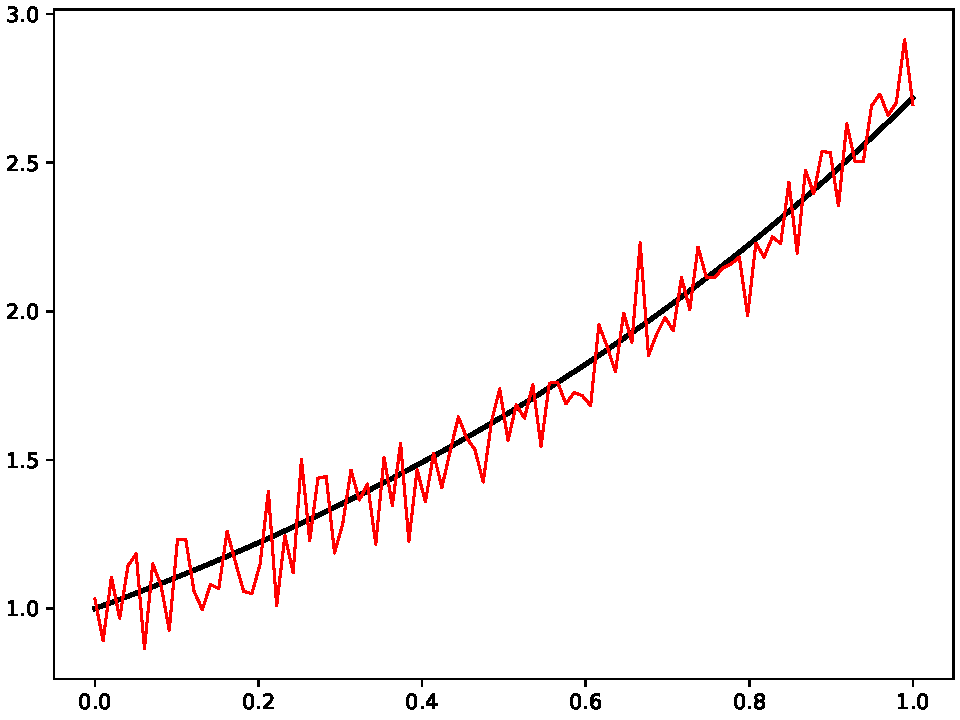
\includegraphics[width=0.5\textwidth]{./figures/exp_with_noise.pdf}
  \caption{An exponential function with random noise.}\label{fig:exp_with_noise}
\end{figure}

An example of a random paper is here~\cite{ChOlSe_2021_lsrbm}.

\bibliographystyle{siamplain}
\bibliography{refs_randomnoise.bib}

\end{document}
